Après optimisation de nos hyper-paramètres, on conclut que le modèle ayant le mieux performer en validation est un modèle avec un objet de compte binaire (0 ou 1) qui utilise des 1-gramme et qui conserve une fréquence minimale de 2 mots. Le modèle de classification utilisé est une régression logistique avec une pénalité de choix de paramètres \emph{L1}:

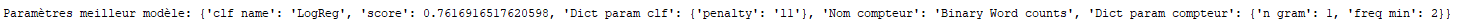
\includegraphics[width=\linewidth,height=1cm,keepaspectratio]{images/dict_meilleur_model}

On peut évaluer notre modèle en calculant le score qu'on obtiendrait sur 80\% de notre corpus d'entraînement qui sert d'entraînement, et 20 \% qui sert de test.
On entraîne donc ce modèle sur l'ensemble de nos données d'entraînement pour faire des prédictions sur notre corpus de test.
On procédant ainsi, on obtient la matrice de confusion présentée dans la figure \ref{fig:full_confusion}.

\begin{figure}
	\caption{Matrice de confusion pour paramètres complets}
	\centering
	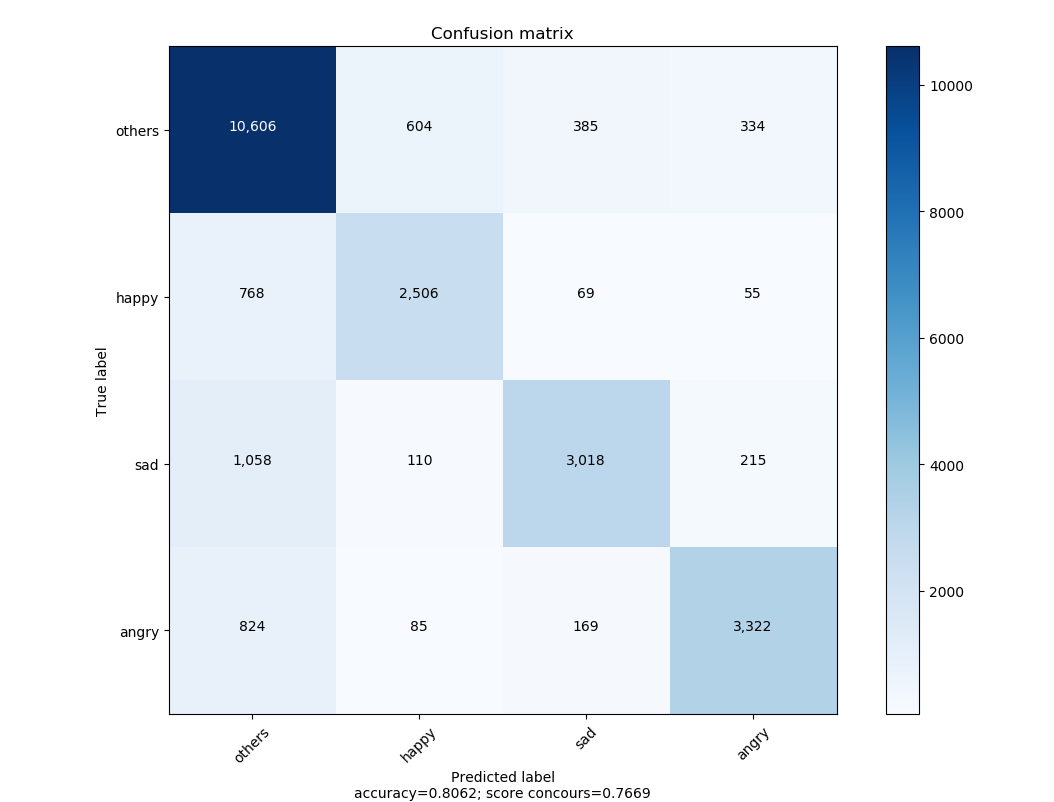
\includegraphics[width=\linewidth,keepaspectratio]{images/confusion_matrix_avec_features}
	\label{fig:full_confusion}
\end{figure}

On peut voir que notre score F1 (utilisé pour l'évaluation du concours) de 0.7669 est quand même assez haut. 
On remarque que la plupart des erreurs faites sont de prédire \emph{happy}, \emph{sad} et \emph{angry} comme étant \emph{others}. Cette caractéristique serait peut être même avantageuse pour le concours puisque la proportion d'échanges de textos considérés comme étant \emph{Others} est bien plus élevée dans le corpus d'évaluation du concours que dans le jeu d'entraînement fourni avec l'énoncé.

De plus, la confusion entre \emph{sad} et \emph{angry} est un peu plus élevée qu'entre les autres paires d'émotions puisqu'on a pu voir que les deux sont à caractère négatif et partagent sans doute certains attributs.

On peut également observer la matrice de confusion lorsque l'on n'ajoute pas les variables supplémentaires décrites précédemment dans la figure \ref{fig:partial_confusion}.

\begin{figure}
	\caption{Matrice de confusion sans paramètres additionnels}
	\centering
	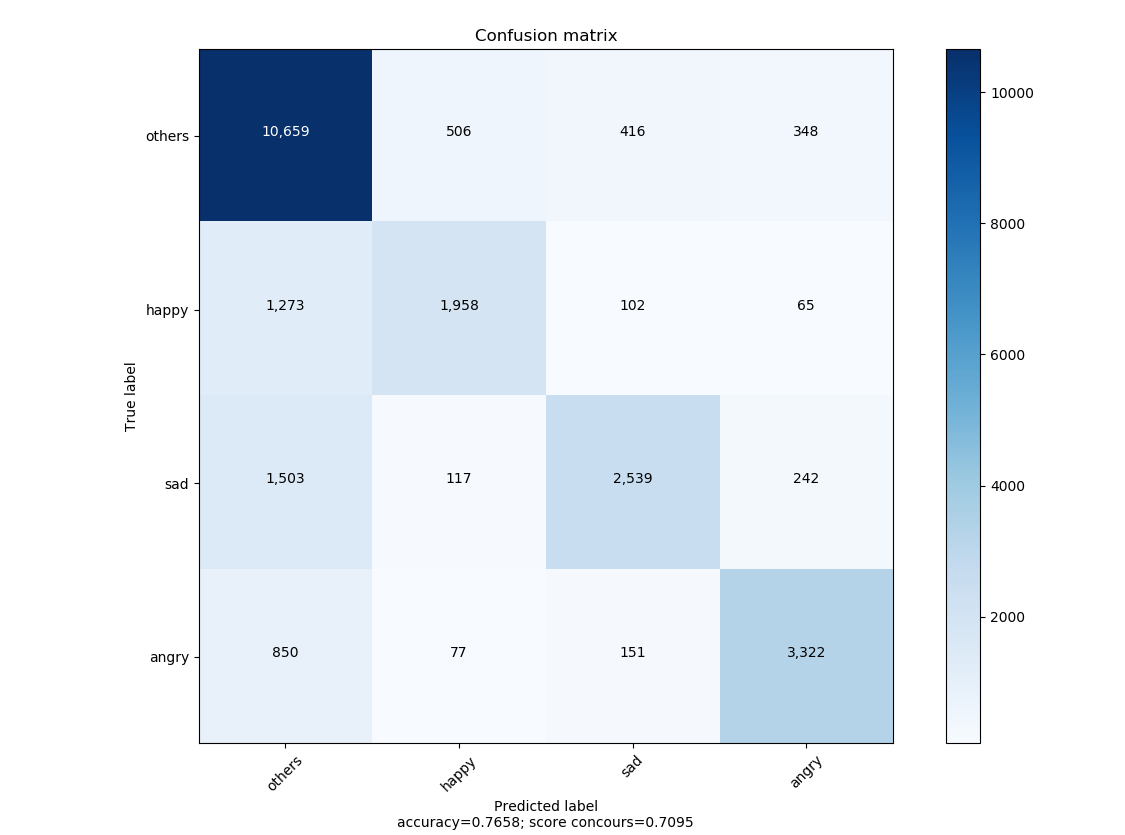
\includegraphics[width=\linewidth,keepaspectratio]{images/confusion_matrix_sans_features}
	\label{fig:partial_confusion}
\end{figure}

On voit tout de suite que le score est beaucoup moins bon (0.7095 au lieu de 0.7669). On remarque aussi que beaucoup plus de classes \emph{happy} et \emph{sad} ont été prédites comme étant \emph{others} (768 à 1273 et 1058 à 1503). Pour ce qui est des données de classe \emph{angry}, les nombres changent très peu. On peut  supposer qu'il y a très peu d'emojis et de binettes dans notre corpus de test pour la classe \emph{angry}.

Encore une fois, on peut supposer que notre modèle avec les variables ajoutées est meilleur que celui sans celles-ci, à cause du meilleur score F1. On peut également comparer notre score aux meilleurs scores soumis à la compétition:

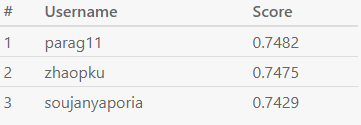
\includegraphics[width=\linewidth,height=4cm,keepaspectratio]{images/meilleurs_scores}

On peut conclure qu'un score de 0.7669 en simulation de test est donc très bon. Il est toutefois difficile de bien comparer notre modèle à ceux qui ont été soumis puisque la répartition des classes n'est pas la même dans le corpus à prédire. Le fichier de test que nous avons utilisé avait environ 16.6\% de \emph{happy}, \emph{sad}, \emph{angry} et 50\% de \emph{others}, alors que le fichier à prédire a des proportions de 4\% pour chacune des trois classes minoritaires et 88\% de \emph{other}. 

On peut quand même être réellement satisfait du résultat obtenu par notre approche, surtout en considérant que la majorité de nos erreurs consistaient à prédire \emph{others} alors que nous faisions face à un échange avec un autre sentiment.